\documentclass[8pt]{beamer}

% Beamer style
%\usetheme[secheader]{Madrid}
% \usetheme{CambridgeUS}
\useoutertheme{infolines}
\usecolortheme[rgb={0.65,0.15,0.25}]{structure}
% \usefonttheme[onlymath]{serif}
\beamertemplatenavigationsymbolsempty
%\AtBeginSubsection

% Packages
%\usepackage[french]{babel}
\usepackage[latin1]{inputenc}
\usepackage{color}
% \usepackage[dvipsnames]{xcolor}
\usepackage{xspace}
\usepackage{dsfont, stmaryrd}
\usepackage{amsmath, amsfonts, amssymb, stmaryrd, mathabx}
\usepackage{epsfig}
\usepackage{tikz}
\usepackage{url}
% \usepackage{ulem}
\usepackage{/home/robin/LATEX/Biblio/astats}
%\usepackage[all]{xy}
\usepackage{graphicx}

% Maths
% \newtheorem{theorem}{Theorem}
% \newtheorem{definition}{Definition}
\newtheorem{proposition}{Proposition}
% \newtheorem{assumption}{Assumption}
% \newtheorem{algorithm}{Algorithm}
% \newtheorem{lemma}{Lemma}
% \newtheorem{remark}{Remark}
% \newtheorem{exercise}{Exercise}
% \newcommand{\propname}{Prop.}
% \newcommand{\proof}{\noindent{\sl Proof:}\quad}
% \newcommand{\eproof}{$\blacksquare$}

% \setcounter{secnumdepth}{3}
% \setcounter{tocdepth}{3}
\newcommand{\pref}[1]{\ref{#1} p.\pageref{#1}}
\newcommand{\qref}[1]{\eqref{#1} p.\pageref{#1}}

% Colors : http://latexcolor.com/
\definecolor{darkred}{rgb}{0.65,0.15,0.25}
\definecolor{darkgreen}{rgb}{0,0.4,0}
\definecolor{darkred}{rgb}{0.65,0.15,0.25}
\definecolor{amethyst}{rgb}{0.6, 0.4, 0.8}
\definecolor{asparagus}{rgb}{0.53, 0.66, 0.42}
\definecolor{applegreen}{rgb}{0.55, 0.71, 0.0}
\definecolor{awesome}{rgb}{1.0, 0.13, 0.32}
\definecolor{blue-green}{rgb}{0.0, 0.87, 0.87}
\definecolor{red-ggplot}{rgb}{0.52, 0.25, 0.23}
\definecolor{green-ggplot}{rgb}{0.42, 0.58, 0.00}
\definecolor{purple-ggplot}{rgb}{0.34, 0.21, 0.44}
\definecolor{blue-ggplot}{rgb}{0.00, 0.49, 0.51}

% Commands
\newcommand{\backupbegin}{
   \newcounter{finalframe}
   \setcounter{finalframe}{\value{framenumber}}
}
\newcommand{\backupend}{
   \setcounter{framenumber}{\value{finalframe}}
}
\newcommand{\emphase}[1]{\textcolor{darkred}{#1}}
\newcommand{\comment}[1]{\textcolor{gray}{#1}}
\newcommand{\paragraph}[1]{\textcolor{darkred}{#1}}
\newcommand{\refer}[1]{{\small{\textcolor{gray}{{\cite{#1}}}}}}
\newcommand{\Refer}[1]{{\small{\textcolor{gray}{{[#1]}}}}}
\newcommand{\goto}[1]{{\small{\textcolor{blue}{[\#\ref{#1}]}}}}
\renewcommand{\newblock}{}

\newcommand{\tabequation}[1]{{\medskip \centerline{#1} \medskip}}
% \renewcommand{\binom}[2]{{\left(\begin{array}{c} #1 \\ #2 \end{array}\right)}}

% Variables 
\newcommand{\Abf}{{\bf A}}
\newcommand{\Beta}{\text{B}}
\newcommand{\Bcal}{\mathcal{B}}
\newcommand{\Bias}{\xspace\mathbb B}
\newcommand{\Cor}{{\mathbb C}\text{or}}
\newcommand{\Cov}{{\mathbb C}\text{ov}}
\newcommand{\cl}{\text{\it c}\ell}
\newcommand{\Ccal}{\mathcal{C}}
\newcommand{\cst}{\text{cst}}
\newcommand{\Dcal}{\mathcal{D}}
\newcommand{\Ecal}{\mathcal{E}}
\newcommand{\Esp}{\xspace\mathbb E}
\newcommand{\Espt}{\widetilde{\Esp}}
\newcommand{\Covt}{\widetilde{\Cov}}
\newcommand{\Ibb}{\mathbb I}
\newcommand{\Fcal}{\mathcal{F}}
\newcommand{\Gcal}{\mathcal{G}}
\newcommand{\Gam}{\mathcal{G}\text{am}}
\newcommand{\Hcal}{\mathcal{H}}
\newcommand{\Jcal}{\mathcal{J}}
\newcommand{\Lcal}{\mathcal{L}}
\newcommand{\Mt}{\widetilde{M}}
\newcommand{\mt}{\widetilde{m}}
\newcommand{\Nbb}{\mathbb{N}}
\newcommand{\Mcal}{\mathcal{M}}
\newcommand{\Ncal}{\mathcal{N}}
\newcommand{\Ocal}{\mathcal{O}}
\newcommand{\pt}{\widetilde{p}}
\newcommand{\Pt}{\widetilde{P}}
\newcommand{\Pbb}{\mathbb{P}}
\newcommand{\Pcal}{\mathcal{P}}
\newcommand{\Qcal}{\mathcal{Q}}
\newcommand{\qt}{\widetilde{q}}
\newcommand{\Rbb}{\mathbb{R}}
\newcommand{\Sbb}{\mathbb{S}}
\newcommand{\Scal}{\mathcal{S}}
\newcommand{\st}{\widetilde{s}}
\newcommand{\St}{\widetilde{S}}
\newcommand{\Tcal}{\mathcal{T}}
\newcommand{\todo}{\textcolor{red}{TO DO}}
\newcommand{\Ucal}{\mathcal{U}}
\newcommand{\Un}{\math{1}}
\newcommand{\Vcal}{\mathcal{V}}
\newcommand{\Var}{\mathbb V}
\newcommand{\Vart}{\widetilde{\Var}}
\newcommand{\Zcal}{\mathcal{Z}}

% Symboles & notations
\newcommand\independent{\protect\mathpalette{\protect\independenT}{\perp}}\def\independenT#1#2{\mathrel{\rlap{$#1#2$}\mkern2mu{#1#2}}} 
\renewcommand{\d}{\text{\xspace d}}
\newcommand{\gv}{\mid}
\newcommand{\ggv}{\, \| \, }
% \newcommand{\diag}{\text{diag}}
\newcommand{\card}[1]{\text{card}\left(#1\right)}
\newcommand{\trace}[1]{\text{tr}\left(#1\right)}
\newcommand{\matr}[1]{\boldsymbol{#1}}
\newcommand{\matrbf}[1]{\mathbf{#1}}
\newcommand{\vect}[1]{\matr{#1}} %% un peu inutile
\newcommand{\vectbf}[1]{\matrbf{#1}} %% un peu inutile
\newcommand{\trans}{\intercal}
\newcommand{\transpose}[1]{\matr{#1}^\trans}
\newcommand{\crossprod}[2]{\transpose{#1} \matr{#2}}
\newcommand{\tcrossprod}[2]{\matr{#1} \transpose{#2}}
\newcommand{\matprod}[2]{\matr{#1} \matr{#2}}
\DeclareMathOperator*{\argmin}{arg\,min}
\DeclareMathOperator*{\argmax}{arg\,max}
\DeclareMathOperator{\sign}{sign}
\DeclareMathOperator{\tr}{tr}
\newcommand{\ra}{\emphase{$\rightarrow$} \xspace}

% Hadamard, Kronecker and vec operators
\DeclareMathOperator{\Diag}{Diag} % matrix diagonal
\DeclareMathOperator{\diag}{diag} % vector diagonal
\DeclareMathOperator{\mtov}{vec} % matrix to vector
\newcommand{\kro}{\otimes} % Kronecker product
\newcommand{\had}{\odot}   % Hadamard product

% TikZ
\newcommand{\nodesize}{2em}
\newcommand{\edgeunit}{2.5*\nodesize}
\newcommand{\edgewidth}{1pt}
\tikzstyle{node}=[draw, circle, fill=black, minimum width=.75\nodesize, inner sep=0]
\tikzstyle{square}=[rectangle, draw]
\tikzstyle{param}=[draw, rectangle, fill=gray!50, minimum width=\nodesize, minimum height=\nodesize, inner sep=0]
\tikzstyle{hidden}=[draw, circle, fill=gray!50, minimum width=\nodesize, inner sep=0]
\tikzstyle{hiddenred}=[draw, circle, color=red, fill=gray!50, minimum width=\nodesize, inner sep=0]
\tikzstyle{observed}=[draw, circle, minimum width=\nodesize, inner sep=0]
\tikzstyle{observedred}=[draw, circle, minimum width=\nodesize, color=red, inner sep=0]
\tikzstyle{eliminated}=[draw, circle, minimum width=\nodesize, color=gray!50, inner sep=0]
\tikzstyle{empty}=[draw, circle, minimum width=\nodesize, color=white, inner sep=0]
\tikzstyle{blank}=[color=white]
\tikzstyle{nocircle}=[minimum width=\nodesize, inner sep=0]

\tikzstyle{edge}=[-, line width=\edgewidth]
\tikzstyle{edgebendleft}=[-, >=latex, line width=\edgewidth, bend left]
\tikzstyle{edgebendright}=[-, >=latex, line width=\edgewidth, bend right]
\tikzstyle{lightedge}=[-, line width=\edgewidth, color=gray!50]
\tikzstyle{lightedgebendleft}=[-, >=latex, line width=\edgewidth, bend left, color=gray!50]
\tikzstyle{lightedgebendright}=[-, >=latex, line width=\edgewidth, bend right, color=gray!50]
\tikzstyle{edgered}=[-, line width=\edgewidth, color=red]
\tikzstyle{edgebendleftred}=[-, >=latex, line width=\edgewidth, bend left, color=red]
\tikzstyle{edgebendrightred}=[-, >=latex, line width=\edgewidth, bend right, color=red]

\tikzstyle{arrow}=[->, >=latex, line width=\edgewidth]
\tikzstyle{arrowbendleft}=[->, >=latex, line width=\edgewidth, bend left]
\tikzstyle{arrowbendright}=[->, >=latex, line width=\edgewidth, bend right]
\tikzstyle{arrowred}=[->, >=latex, line width=\edgewidth, color=red]
\tikzstyle{arrowbendleftred}=[->, >=latex, line width=\edgewidth, bend left, color=red]
\tikzstyle{arrowbendrightred}=[->, >=latex, line width=\edgewidth, bend right, color=red]
\tikzstyle{arrowblue}=[->, >=latex, line width=\edgewidth, color=blue]
\tikzstyle{dashedarrow}=[->, >=latex, dashed, line width=\edgewidth]
\tikzstyle{dashededge}=[-, >=latex, dashed, line width=\edgewidth]
\tikzstyle{dashededgebendleft}=[-, >=latex, dashed, line width=\edgewidth, bend left]
\tikzstyle{lightarrow}=[->, >=latex, line width=\edgewidth, color=gray!50]

\newcommand{\dN}{\Delta N}
\newcommand{\dtau}{\Delta \tau}

% Directory
\newcommand{\fignet}{/home/robin/RECHERCHE/RESEAUX/EXPOSES/FIGURES}

%====================================================================
%====================================================================

%====================================================================
%====================================================================
\begin{document}
%====================================================================
%====================================================================

%====================================================================
\title[An exchangeable model for bipartite networks]{An exchangeable model for (ecological) bipartite networks}

\author[S. Robin]{S. Robin}

\institute[Sorbonne universit�]{\normalsize{Sorbonne universit�}}

\date[Mar. 2022]{ ~ \\  ~ \\ 
  joint work with S. Ouadah (AgroParisTech), P. Latouche (universit� Paris Cit�) \\ \medskip
  and T. Le Minh, S. Donnet (INRAE), F. Massol (CNRS, Lille)  \\ 
  \bigskip ~ \\ \bigskip
  WG on Risk, ESSEC, Mar. 2022}

%====================================================================
%====================================================================
\maketitle

%====================================================================
%====================================================================
\section*{Introduction}
%====================================================================
\subsection*{Bipartite networks}
%====================================================================
\frame{\frametitle{Bipartite networks} 

  \begin{tabular}{cc}
    \hspace{-.04\textwidth}
    \begin{tabular}{p{.55\textwidth}}
      \paragraph{Bipartite networks} describe the connections between two set of entities
      \begin{itemize}
      \item authors / publications, 
      \item actors / movies, 
      \item hosts / parasites, 
      \item plants / pollinators, 
      \item etc.
      \end{itemize}
      
      \bigskip \bigskip \pause
      \paragraph{Example:} 
      \begin{description}
       \item[Top:] Plants ($\circ$) 
       \item[Bottom:] Pollinators ($\square$)
      \end{description}
      Zackenberg network from \refer{OBE08,SRO16,CRR18}:  
      $$
      m = 17, \quad n = 24
      $$
    \end{tabular}
    & 
    \hspace{-.05\textwidth}
    \begin{tabular}{c}
      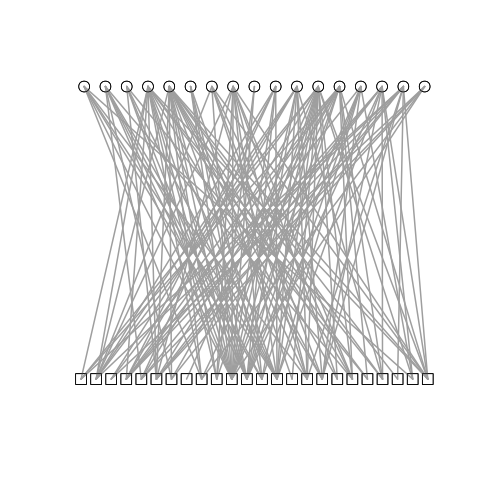
\includegraphics[width=.35\textwidth, trim=0 50 0 50]{\fignet/FigBEDD-Zackenberg-1996_12-Net1} \\
      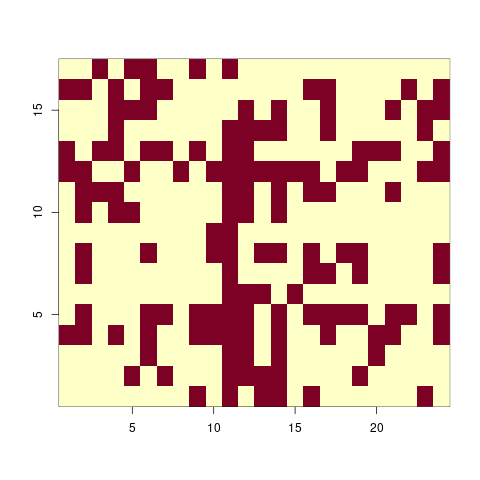
\includegraphics[width=.35\textwidth, trim=0 10 10 50, clip]{\fignet/FigBEDD-Zackenberg-1996_12-Adj1}
    \end{tabular}
  \end{tabular}

}

%====================================================================
\subsection*{Exchangeability}
%====================================================================
\frame{\frametitle{Species exchangeability} 

  \begin{tabular}{cc}
    \hspace{-.04\textwidth}
    \begin{tabular}{p{.55\textwidth}}
      \paragraph{Aim.} Describe the global organization ('topology') of the network to
      \begin{itemize}
       \item better understand the behavior of the ecosystem, 
       \item or predict its response to a change
      \end{itemize}
      
      \bigskip
      \onslide+<2->{
      \bigskip
      \paragraph{Descriptors ('metrics'):} network density, number of connected components, number of 'clusters', 'nestedness', ...}
      
      \bigskip 
      \onslide+<3->{
      \bigskip
      \paragraph{Species exchangeability.} 
      \begin{itemize}
        \item Most descriptors remain unchanged when relabeling the species.
        \item Species are not each considered {\it per se}.
      \end{itemize}}
    \end{tabular}
    & 
    \hspace{-.05\textwidth}
    \begin{overprint}
      \onslide<1-3>
      \begin{tabular}{c}
        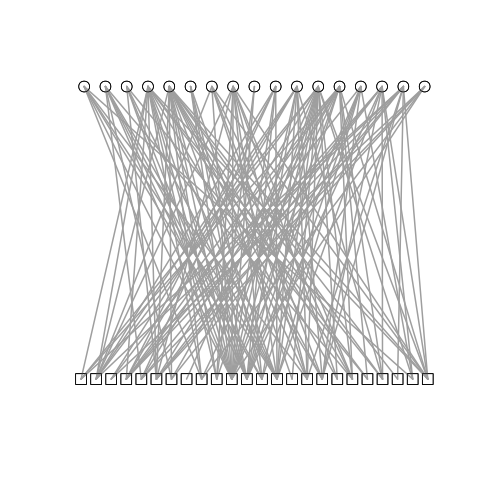
\includegraphics[width=.35\textwidth, trim=0 50 0 50]{\fignet/FigBEDD-Zackenberg-1996_12-Net1} \\
        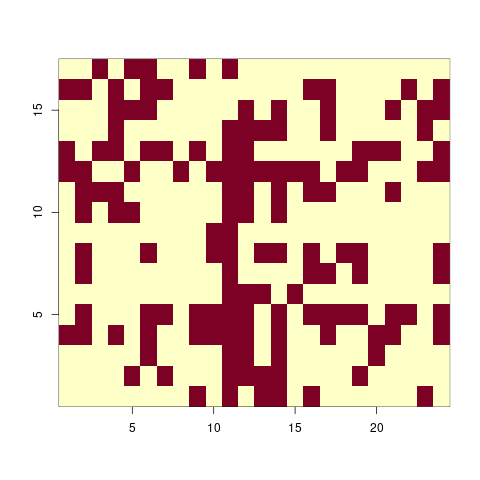
\includegraphics[width=.35\textwidth, trim=0 10 10 50, clip]{\fignet/FigBEDD-Zackenberg-1996_12-Adj1}
      \end{tabular}
      \onslide<4>
      \begin{tabular}{c}
        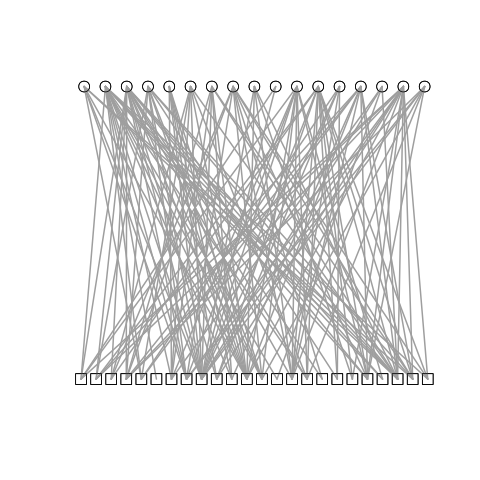
\includegraphics[width=.35\textwidth, trim=0 50 0 50]{\fignet/FigBEDD-Zackenberg-1996_12-Net2} \\
        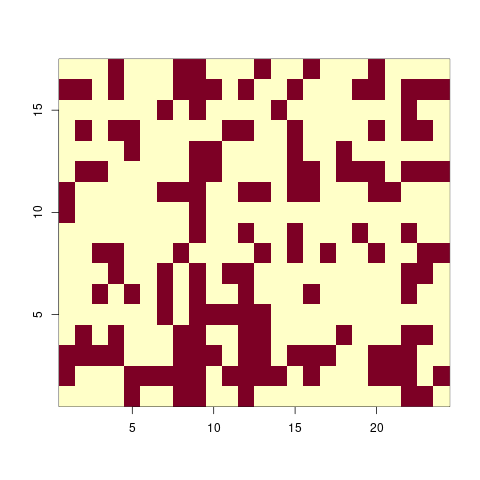
\includegraphics[width=.35\textwidth, trim=0 10 10 50, clip]{\fignet/FigBEDD-Zackenberg-1996_12-Adj2}
      \end{tabular}
      \onslide<5>
      \begin{tabular}{c}
        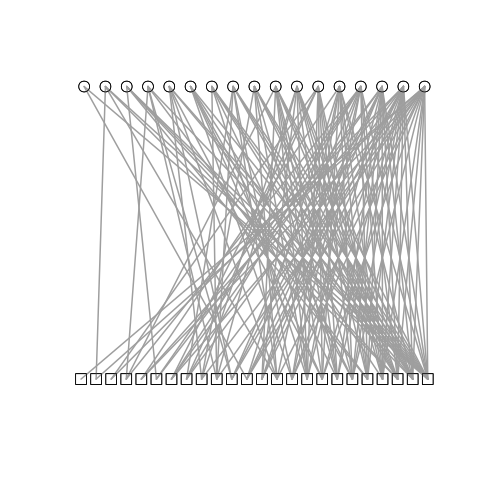
\includegraphics[width=.35\textwidth, trim=0 50 0 50]{\fignet/FigBEDD-Zackenberg-1996_12-Net3} \\
        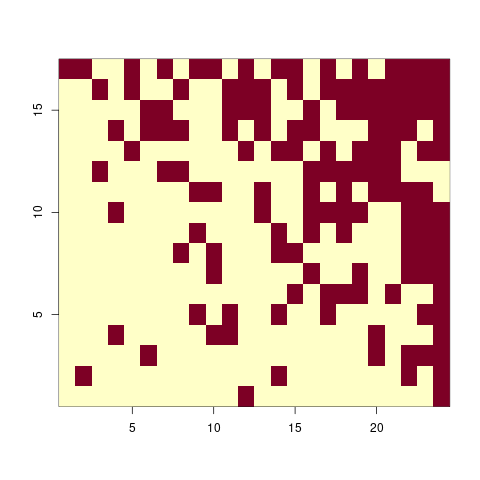
\includegraphics[width=.35\textwidth, trim=0 10 10 50, clip]{\fignet/FigBEDD-Zackenberg-1996_12-Adj3}
      \end{tabular}
      \end{overprint}
  \end{tabular}

}

%====================================================================
%====================================================================
\section{Exchangeable network models}
\frame{\frametitle{Outline} \tableofcontents[currentsection]}
%====================================================================
\frame{\frametitle{Probabilistic formulation} 

  \paragraph{Network.} Can be seen either as
  \begin{itemize}
    \item a graph $\Gcal = (\Vcal = \text{set of vertices}, \Ecal = \text{set of edges} \subset \Vcal \times \Vcal)$, or
    \item an $m \times n$ \emphase{adjacency matrix} $Y = [Y_{ij}]$ where
    $$
    Y_{ij} = 1 \text{ iff the node $i$ is connected with the node $j$} 
    $$
  \end{itemize}

  \bigskip \bigskip \pause
  \paragraph{Probabilistic framework.} The observed network is seen as a \emphase{realization of a random graph} ruled by some \emphase{joint} distribution $p(y)$, that is
  $$
  p(y) = \Pbb\{Y = y\} = \Pbb\{Y_{11} = 1, Y_{12} = 0, \dots Y_{ij} = 1, \dots, Y_{mn} = 0\}
  $$

  \bigskip \bigskip \pause
  \paragraph{Network analysis.}  Classical framework in statistical modelling:
  \begin{itemize}
    \item Questions of (ecological) interest have to be translated into 
    \item Questions about the distribution $p$.
  \end{itemize}
  
}

%====================================================================
\subsection*{Graphon model}
%====================================================================
\frame{\frametitle{Row-column exchangeability (RCE)} 

  \paragraph{Exchangeability assumption.} Species exchangeability means
  \begin{itemize}
    \item Plants can be exchanged with plants, insects can be exchanged with insects, 
    \item That is: for any permutation $\sigma_R$ of the rows and any permutation $\sigma_C$ of the columns:
    $$
    \Pbb(Y = y) = \Pbb(Y = y_{\sigma_R, \sigma_C}).
    $$
  \end{itemize}
  
  \bigskip \bigskip \pause
  \paragraph{Aldous-Hoover representation.} A random graph $Y \sim p$ is RCE iff there exist a \emphase{determistic function} $f$ such that
  \begin{align*}
    Y & = f(T, U_1, \dots U_m, V_1, \dots, V_n, W_{11}, \dots W_{mn}) \\
    \\
%     \text{with } & \{\underset{}{\undebrace{T}}, 
%       \underset{}{\undebrace{U_1, \dots U_m}}, 
%       \underset{}{\undebrace{V_1, \dots, V_n}}, 
%       \underset{}{\undebrace{W_{11}, \dots W_{mn}}}\} \text{ iid } \sim \Ucal[0, 1].
      \text{with } & \left\{ \begin{array}{lll}
             T, & (\text{whole graph}) \\ 
             U_1, \dots U_m, & (\text{rows}) \\ 
             V_1, \dots, V_n, & (\text{columns}) \\ 
             W_{11}, \dots W_{mn} & (\text{edges}) \\ 
             \end{array} \right\}
        \text{ iid } \sim \Ucal[0, 1].
  \end{align*}
}

%====================================================================
\frame{\frametitle{Bipartite $w$-graph} 

  \begin{tabular}{cc}
    \hspace{-.04\textwidth}
    \begin{tabular}{p{.5\textwidth}}
      \paragraph{Model.} 
      \begin{itemize}
        \item Consider a 'graphon' function
        $$
        \phi: [0, 1] \times [0, 1] \mapsto [0, 1],
        $$
        \item draw $(U_1, \dots, U_m)$ iid $\sim \Ucal[0, 1]$,
        \item draw $(V_1, \dots, V_n)$ iid $\sim \Ucal[0, 1]$,
        \item draw $(Y_{11}, \dots, Y_{mn})$ independently:
        $$
        \Pbb\{Y_{ij} = 1\} = \phi(U_i, V_j).
        $$
      \end{itemize}
      
      \bigskip
      \onslide+<2->{
      \paragraph{Latent block-model \refer{GoN05}.} Block-wise constant function $\phi$.
      }
    \end{tabular}
    & 
    \hspace{-.05\textwidth}
    \begin{tabular}{p{.5\textwidth}}
      \begin{overprint}
        \onslide<1>
        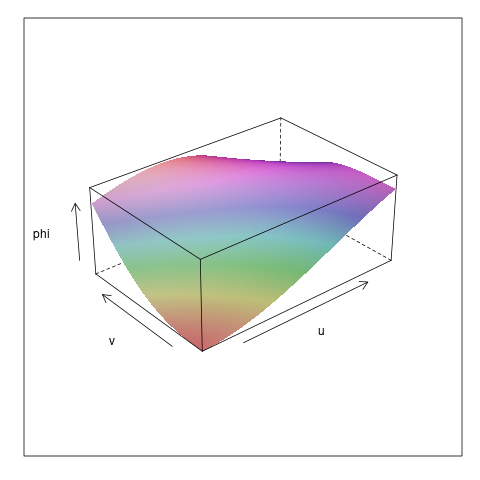
\includegraphics[width=.45\textwidth, trim=0 50 0 50]{\fignet/FigBEDD-graphon}
        \onslide<2->
        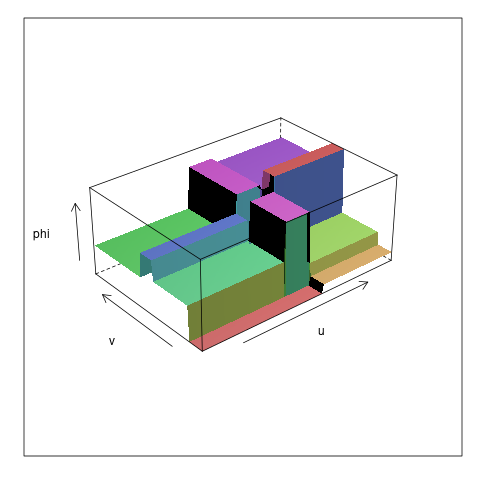
\includegraphics[width=.45\textwidth, trim=0 50 0 50]{\fignet/FigBEDD-LBM}
      \end{overprint}
    \end{tabular}
  \end{tabular}
  
  \onslide+<3>{
  \bigskip \bigskip 
  \paragraph{Dissociated models.} No 'whole graph' random term $T$: 
  \begin{itemize}
   \item Non-overlapping blocks of the adjacency matrix $Y$ are independent.
  \end{itemize}
  }

}

%====================================================================
\subsection*{Expected degree distribution model}
%====================================================================
\frame{\frametitle{Expected degree distribution model} 

  \paragraph{A 'null' model.} Product form $w$-graph:
  $$
  \phi(u, v) = \rho \, f(u) \, g(v)
  $$
  \begin{itemize}
    \item $f: [0, 1] \mapsto \Rbb^+$: row imbalance (\emphase{generalist vs specialist plants}), 
    \item $g: [0, 1] \mapsto \Rbb^+$: column imbalance (\emphase{generalist vs specialist insects}), 
    \item $\rho \in [0, 1]$: network density\footnote{$\int f(u) \d u = 1, \quad \int g(v) \d v = 1, \quad \rho \leq 1/ (\max(f) \max(g))$}.
  \end{itemize}
  
  \bigskip \bigskip \bigskip \pause
  \paragraph{Expected degrees.} % $D^\circ_i =$ degree of top node $i$, $D^\square_j =$ degree of bottom node $j$:
%   $$
%   \Esp(D^\circ_i \mid U_i = u) = n \rho f(u), \qquad \qquad
%   \Esp(D^\square_j \mid V_j = v) = m \rho g(v).
%   $$
  \begin{align*}
    D^\circ_i & = \text{ degree of top node $i$:} &  
    \Esp(D^\circ_i \mid U_i = u) & = n \, \rho \, f(u), \\
    D^\square_j & = \text{ degree of bottom node $j$:} & 
    \Esp(D^\square_j \mid V_j = v) & = m \, \rho \, g(v).
  \end{align*}

  \ra Bipartite version of the expected degree distribution (EDD) model \refer{ChL02}.

}

%==================================================================
\frame{\frametitle{BEDD model}

  \begin{tabular}{cccc}
    & & $g =$ & $g =$ \\
    \multicolumn{2}{l}{
      \hspace{-.04\textwidth}
      \begin{tabular}{p{.4\textwidth}} 
        \begin{itemize}
        \item Only individual effects matter:  $f(U_i)$, $g(V_j)$. \\ ~
        \item No specific interaction $(U_i, V_j)$
        \end{itemize}
      \end{tabular}
%       $\begin{array}{rl}
%         \Pbb\{i \sim j \mid U_i, V_j\} & = \rho \; g(U_i) \; h(V_j) \\ \\
%         \Esp (D_i \mid U_i) & = n \; \rho \; g(U_i) \\ \\
%         \Esp (D_j \mid V_j) & = m \; \rho \; g(V_i) 
%       \end{array}$
    } 
    &
%     \begin{tabular}{p{.2\textwidth}}
%       top degree $\rightarrow$ \\ ~\\
%       bottom deg. $\downarrow$ \\
%     \end{tabular} 
    \begin{tabular}{c} 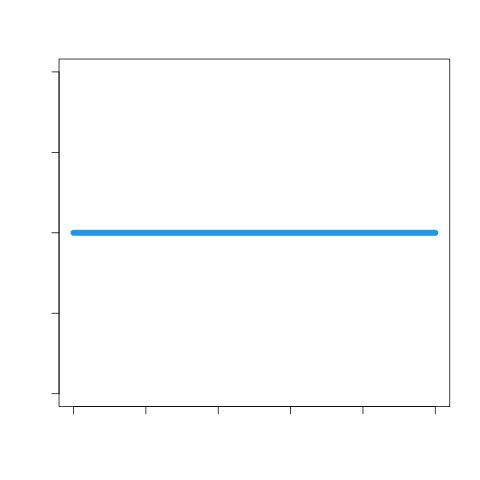
\includegraphics[width=.2\textwidth, trim=20 20 20 20, clip=]{\fignet/FigMotifsBEDD-dist-h10} \end{tabular} &
    \begin{tabular}{c} 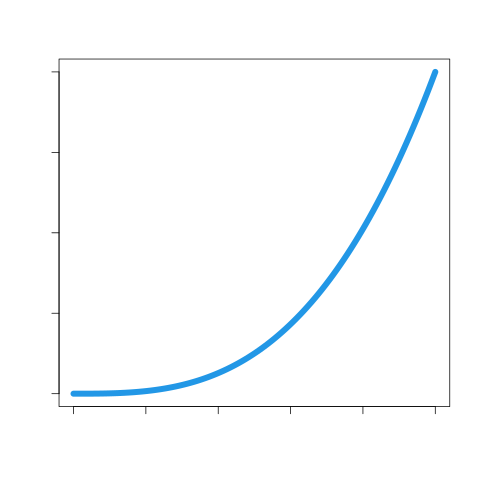
\includegraphics[width=.2\textwidth, trim=20 20 20 20, clip=]{\fignet/FigMotifsBEDD-dist-h40} \end{tabular} \\
    \begin{tabular}{c} $f =$ \end{tabular} &
    \begin{tabular}{c} 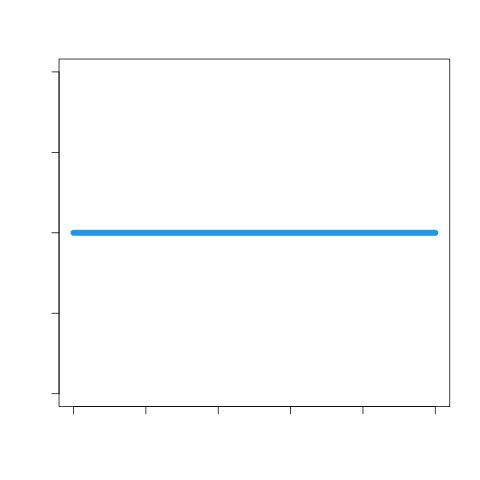
\includegraphics[width=.2\textwidth, trim=20 20 20 20, clip=]{\fignet/FigMotifsBEDD-dist-g10} \end{tabular} &
    \begin{tabular}{c} 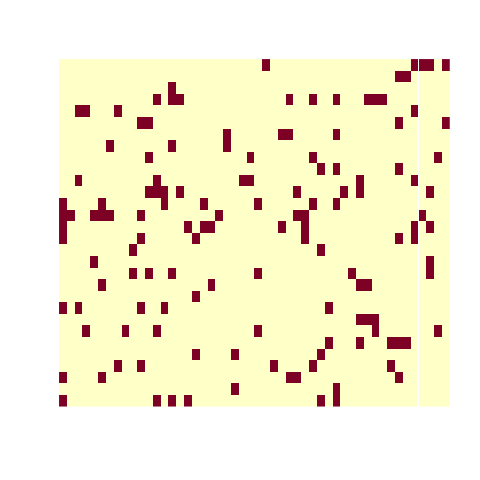
\includegraphics[width=.2\textwidth, trim=20 20 20 20, clip=]{\fignet/FigMotifsBEDD-adj-g10-h10} \end{tabular} &
    \begin{tabular}{c} 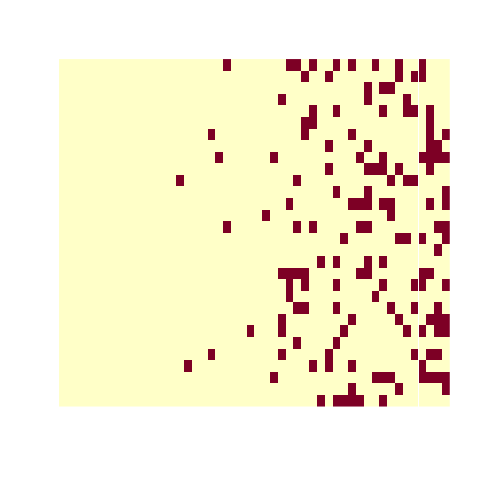
\includegraphics[width=.2\textwidth, trim=20 20 20 20, clip=]{\fignet/FigMotifsBEDD-adj-g10-h40} \end{tabular} \\
    \begin{tabular}{c} $f =$ \end{tabular} &
    \begin{tabular}{c} 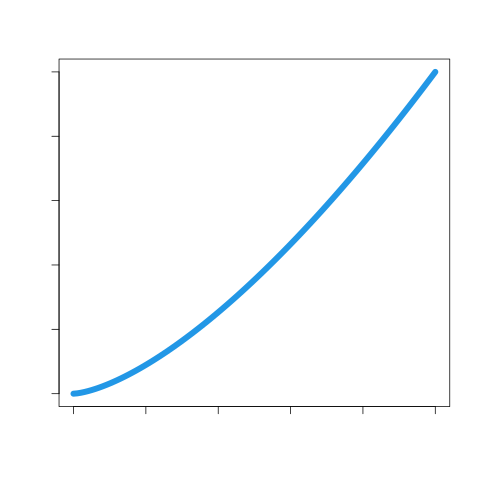
\includegraphics[width=.2\textwidth, trim=20 20 20 20, clip=]{\fignet/FigMotifsBEDD-dist-g25} \end{tabular} &
    \begin{tabular}{c} 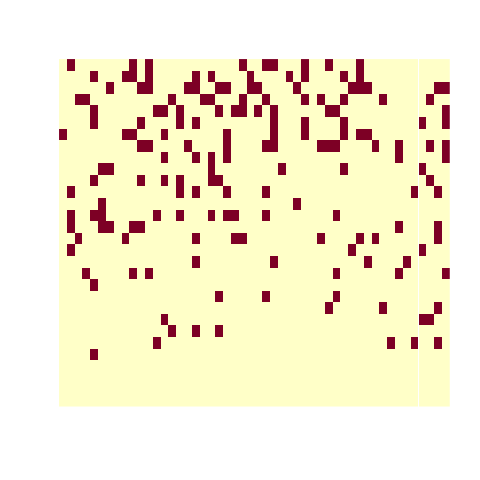
\includegraphics[width=.2\textwidth, trim=20 20 20 20, clip=]{\fignet/FigMotifsBEDD-adj-g25-h10} \end{tabular} &
    \begin{tabular}{c} 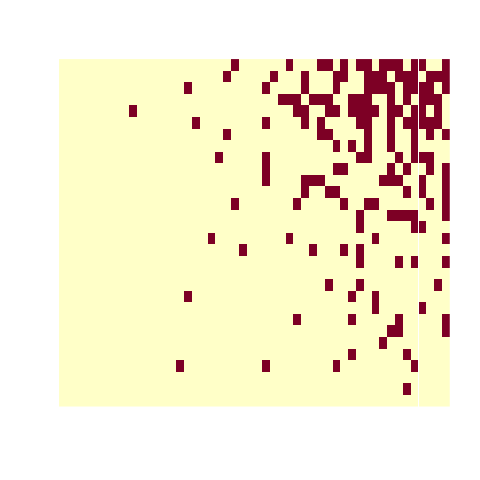
\includegraphics[width=.2\textwidth, trim=20 20 20 20, clip=]{\fignet/FigMotifsBEDD-adj-g25-h40} \end{tabular}
  \end{tabular}

}


%====================================================================
%====================================================================
\section{Network motifs}
\frame{\frametitle{Outline} \tableofcontents[currentsection]}
%====================================================================
\subsection*{Network motifs}
%====================================================================
\frame{\frametitle{Bipartite network motifs}

  \begin{tabular}{ll}
    \hspace{-.04\textwidth}
    \begin{tabular}{p{.45\textwidth}}
      \paragraph{'Meso-scale' analysis.} \refer{SCB19}
      \begin{itemize}
       \item Motifs ='building-blocks'
       \item between local (several nodes) and global (sub-graph)
      \end{itemize}
      \bigskip \bigskip 
      \paragraph{Interest.}
      \begin{itemize}
       \item Generic description of a network
       \item Enables network comparison
       \item Even when the nodes are different
      \end{itemize} \\
      ($+$ 'species-role': see later?) \\ 
      \bigskip \bigskip 
      \paragraph{Existing tool.} 
      \url{bmotif} package \refer{SSS19}: \\
      counts motif occurrences
    \end{tabular}
    &
    \begin{tabular}{p{.45\textwidth}}
      \hspace{-0.075\textwidth}
      \includegraphics[width=.5\textwidth]{\fignet/SCB19-Oikos-Fig3-6motifs} \\      
    \end{tabular} 
  \end{tabular}

}

%==================================================================
\frame{\frametitle{Example}

  \begin{tabular}{ll}
    \begin{tabular}{p{.45\textwidth}}
      \paragraph{Zackenberg network.} \\
      \hspace{-.05\textwidth}
      \includegraphics[width=.45\textwidth, trim=0 50 0 50]{\fignet/Zackenberg-1996_12-red-net} \\
    \end{tabular}
    &
    \begin{tabular}{p{.45\textwidth}}
      \paragraph{Motif counts.}  \\ ~\\ 
      4 nodes (species) \\ 
      \includegraphics[width=.1\textwidth]{\fignet/Zackenberg-1996_12-red-motif5} 
      \includegraphics[width=.1\textwidth]{\fignet/Zackenberg-1996_12-red-motif6} \\ ~\\
      5 nodes \\ 
      \includegraphics[width=.1\textwidth]{\fignet/Zackenberg-1996_12-red-motif9} 
      \includegraphics[width=.1\textwidth]{\fignet/Zackenberg-1996_12-red-motif10} 
      \includegraphics[width=.1\textwidth]{\fignet/Zackenberg-1996_12-red-motif11} 
      \includegraphics[width=.1\textwidth]{\fignet/Zackenberg-1996_12-red-motif12} \\
      \includegraphics[width=.1\textwidth]{\fignet/Zackenberg-1996_12-red-motif13} 
      \includegraphics[width=.1\textwidth]{\fignet/Zackenberg-1996_12-red-motif14} 
      \includegraphics[width=.1\textwidth]{\fignet/Zackenberg-1996_12-red-motif15} 
      \includegraphics[width=.1\textwidth]{\fignet/Zackenberg-1996_12-red-motif16} 
    \end{tabular}  
    ~ \\
    \hline
    \\
    \begin{tabular}{p{.45\textwidth}}
      top 'stars' (plants) \\
      \includegraphics[width=.1\textwidth]{\fignet/Zackenberg-1996_12-red-motif1} 
      \includegraphics[width=.1\textwidth]{\fignet/Zackenberg-1996_12-red-motif2} 
      \includegraphics[width=.1\textwidth]{\fignet/Zackenberg-1996_12-red-motif7} 
      \includegraphics[width=.1\textwidth]{\fignet/Zackenberg-1996_12-red-motif17} 
    \end{tabular}
    &    
    \begin{tabular}{p{.45\textwidth}}
      bottom 'stars' (pollinators) \\
      \includegraphics[width=.1\textwidth]{\fignet/Zackenberg-1996_12-red-motif1} 
      \includegraphics[width=.1\textwidth]{\fignet/Zackenberg-1996_12-red-motif3} 
      \includegraphics[width=.1\textwidth]{\fignet/Zackenberg-1996_12-red-motif4} 
      \includegraphics[width=.1\textwidth]{\fignet/Zackenberg-1996_12-red-motif8} 
    \end{tabular}
  \end{tabular}
  
}

%====================================================================
\subsection*{Motif count}
%==================================================================
\frame{\frametitle{Counting motifs}

  \hspace{-.05\textwidth}
  \begin{tabular}{ll}
    \begin{tabular}{p{.4\textwidth}}
      \paragraph{Number of positions.}
      \begin{itemize}
       \item Choose $p$ nodes among $m$
       \item Choose $q$ nodes among $n$
       \item Try all {\sl automorphisms} 
      \end{itemize}
      $$
      c_s := 
      \left(\begin{array}{c}m \\ p\end{array}\right)
      \times \left(\begin{array}{c}n \\ q\end{array}\right)
      \times r_s
      $$ 
      ~ \\ ~ \\
    \end{tabular}
    & \pause
    \begin{tabular}{c}
      \paragraph{Automorphisms =} non-redundant permutations \\
      \includegraphics[width=.1\textwidth]{\fignet/FigMotifsBEDD-motif9-automorphism1}
      \includegraphics[width=.1\textwidth]{\fignet/FigMotifsBEDD-motif9-automorphism2}
      \includegraphics[width=.1\textwidth]{\fignet/FigMotifsBEDD-motif9-automorphism3} \\
      \includegraphics[width=.1\textwidth]{\fignet/FigMotifsBEDD-motif9-automorphism4}
      \includegraphics[width=.1\textwidth]{\fignet/FigMotifsBEDD-motif9-automorphism5}
      \includegraphics[width=.1\textwidth]{\fignet/FigMotifsBEDD-motif9-automorphism6} 
    \end{tabular} 
  \end{tabular}
  
  \bigskip \bigskip \pause
  \paragraph{Motif count.} Try all positions $\alpha = 1, \dots c_s$, define 
  $$
  Y_{s\alpha} = 1 \text{ if match,} \qquad 0 \text{ otherwise},
  $$
  then count the number of matches:
  $$
  N_s = \sum_\alpha Y_{s\alpha}
  $$
  \ra Motif frequency: $F_s := N_s / c_s$
  
}

%==================================================================
\frame{\frametitle{Motif probability}

  \paragraph{Occurrence probability $\overline{\phi}_s = \Pbb\{Y_{s\alpha} = 1\}$.} Under the BEDD model:
  \begin{align*}
    \overline{\phi}_s 
    & :=
    \Pbb_{BEDD}\left(
    \includegraphics[width=.06\textwidth, trim=100 200 100 0]{\fignet/FigMotifsBEDD-motif9} 
    \right)
    \; = \; 
    \frac{
    \onslide+<2->{
      \overset{\text{top stars: $\lambda_d$}}{\overbrace{
      \Pbb\left(\includegraphics[width=.05\textwidth, trim=100 200 100 0]{\fignet/FigMotifsBEDD-motif9-top1}\right) % \times 
      \Pbb\left(\includegraphics[width=.05\textwidth, trim=100 200 100 0]{\fignet/FigMotifsBEDD-motif9-top1}\right) % \times 
      \Pbb\left(\includegraphics[width=.05\textwidth, trim=100 200 100 0]{\fignet/FigMotifsBEDD-motif9-top2}\right)   }}
    }
    \onslide+<3->{
      \times
      \overset{\text{bottom stars: $\gamma_d$}}{\overbrace{
      \Pbb\left(\includegraphics[width=.05\textwidth, trim=100 200 100 0]{\fignet/FigMotifsBEDD-motif9-bottom1}\right) % \times
      \Pbb\left(\includegraphics[width=.05\textwidth, trim=100 200 100 0]{\fignet/FigMotifsBEDD-motif9-bottom3}\right)
      }}
    }
    }{
    \onslide+<4->{
      \underset{\text{edges: $\rho$}}{\underbrace{
      \left(\Pbb\left(\includegraphics[width=.05\textwidth, trim=100 200 100 0]{\fignet/FigMotifsBEDD-motif9-top1}\right)\right)^4
      }}
    }
    } 
    \\
    \onslide+<5->{
    & =
    \frac{\rho^2 \lambda_2 \rho \gamma_3}{\rho^4}
    \qquad =
    \frac{\lambda_2 \gamma_3}{\rho}
    \qquad \qquad \text{where } \lambda_d = \rho^d \int f^d(u) \d u, \qquad \gamma_d = \rho^d \int g^d(v) \d v
    }
  \end{align*}

  \onslide+<6->{\bigskip \bigskip 
  \paragraph{Estimated probability.} 
  $$
  \overline{\phi}_s := \frac{\lambda_2 \gamma_3}{\rho}
  \qquad \rightarrow \qquad 
  \overline{F}_s := \frac{\Lambda_2 \Gamma_3}{R}
  $$
  where $\Lambda_2$, $\Gamma_3$, $R =$ empirical frequencies of top stars, bottom stars and edges.
  }
}

%====================================================================
\subsection*{Motif distribution}
%==================================================================
\frame{\frametitle{Distribution of the count}

  \paragraph{Moments:}
  \begin{itemize}
  \item \emphase{Mean:} $\Esp_{BEDD}(N_s) = c_s \times \overline{\phi}_s$ \\ ~
  \item \emphase{Variance:} Requires to evaluate $\displaystyle{\Esp_{BEDD}(N_s ^2) = \Esp_{BEDD}\left(\sum_\alpha Y_{s\alpha} \right)^2}$ \\
  \ra Need to account for overlap between positions ({\sl super-motifs}: \refer{PDK08}) \\ ~
  \item \emphase{Covariance:} Same game to compute $\Cov(N_s, N_{s'})$
  \end{itemize}

  \bigskip \bigskip \pause
  \paragraph{Asymptotic normality for non-star motifs \refer{OLR22}.} Under BEDD (and sparsity conditions):
  $$
  (F_s - \overline{F}_s) \left/ \sqrt{\widehat{\Var}(F_s)} \right. \quad \overset{m, n \rightarrow \infty}{\longrightarrow} \quad \Ncal(0, 1)
  $$ \pause
  Proof: 
  \begin{itemize}
   \item decompose 
   $$
   F_s - \overline{F}_s 
   = \underset{\text{random fluctuations}}{\underbrace{(F_s - \phi_s)}} 
   + \underset{\text{null under BEDD}}{\underbrace{(\phi_s - \overline{\phi}_s)}}  
   + \underset{\text{estimation error } \rightarrow 0}{\underbrace{(\overline{\phi}_s - \overline{F}_s)}}, 
   $$
   \item construct a counting martingale \refer{GaL17b} for $(F_s - \phi_s)$ + consistent estimate of $\widehat{\Var}(F_s)$.
  \end{itemize}

}

%====================================================================
\subsection*{Tests}
%==================================================================
\frame{\frametitle{Goodness-of-fit (GOF) of the BEDD model}

  \hspace{-.05\textwidth}
  \begin{tabular}{ll}
    \begin{tabular}{p{.5\textwidth}}
      \onslide+<1->{\paragraph{Raw test statistic:}
      $$
      T_s = \frac{N_s - \widehat{\Esp} N_s}{\sqrt{\widehat{\Var} N_s}}
      $$ \\ 
      }
      \onslide+<2->{
      \paragraph{Corrected statistic:} accounts for the estimation error in $\widehat{\Esp} N$
      $$
      T'_s = \frac{N_s - (\widehat{\Esp} N_s - \emphase{\widehat{\Bias}(\widehat{\Esp} N_s)})}{\sqrt{\emphase{\widehat{\Var} (N_s - \widehat{\Esp} N_s)}}}
      $$ \\ 
      }
      \onslide+<3>{\paragraph{Cholevski      
      \footnote{$\Sigma = P \Lambda P^\intercal$, $\Sigma = P \Lambda^{-1/2} P^\intercal$} 
      transformation:} accounts for the correlation between the counts
      $$
      \Sigma_{s, s'} = \Cov(N_s - \widehat{\Esp} N_s, N_{s'} - \widehat{\Esp} N_{s'})
      $$
      $$
      T'' = \emphase{\widehat{\Sigma}^{-1/2}}
      \left[N_s - (\widehat{\Esp} N_s - \widehat{\Bias}(\widehat{\Esp} N_s))\right]
      $$
      }
    \end{tabular}
    &
    \begin{tabular}{p{.4\textwidth}}
      \hspace{-.05\textwidth}
      \onslide+<1->{\paragraph{Zackenberg network.} ~ \\}
      \begin{overprint}
        \onslide<1>
        \includegraphics[width=.4\textwidth]{\fignet/Zackenberg-1996_12-red-StatCount}
        \onslide<2>
        \includegraphics[width=.4\textwidth]{\fignet/Zackenberg-1996_12-red-NormStatCount}
        \onslide<3>
        \includegraphics[width=.4\textwidth]{\fignet/Zackenberg-1996_12-red-CholNormStat}
      \end{overprint}
    \end{tabular} 
  \end{tabular}

}

%====================================================================
\frame{\frametitle{Network comparison} 

  \bigskip
  \paragraph{Same degree imbalance for top nodes.} 
  \begin{itemize}
   \item Consider two networks $G^A \sim BEDD(\rho^A, f^A, g^A)$ and $G^B \sim BEDD(\rho^B, f^B, g^B)$ and
   $$
   H_0 = \{f^A = f^B\}
   $$ \pause
%    \item Under $H_0$, $\gamma_d^A/(\rho^A)^d = \gamma_d^B/(\rho^B)^d$, so we may define 
%    $$
%    \widehat{\Esp}_0({\Gamma}_d^A) = \left(\frac{F_1^A}{F_1^B}\right)^d \Gamma_d^B
%    \qquad \qquad (\text{idem for } \widehat{\Esp}_0({\Gamma}_d^B))
%    $$
%    to get estimates of  ${\Esp}_0(F_s^A)$, ${\Var}_0(F_s^A)$, ${\Esp}_0(F_s^B)$, ${\Var}_0(F_s^B)$, ... \\ ~ \\ ~ \pause
   \item Under $H_0$ \refer{OLR22}
   $$
   W_s = \frac{\left(F_s^A - \widehat{\Esp}_0(F_s^A)\right) - \left(F_s^B - \widehat{\Esp}_0(F_s^B)\right)}{\sqrt{\widehat{\Var}_0(F_s^A) + \widehat{\Var}_0(F_s^B)}}
   \overset{D}{\longrightarrow} \Ncal(0, 1)
   $$
  \end{itemize}

% }
% 
% %====================================================================
% \frame{\frametitle{Plant-pollinator vs Plant-seed disperser} 

  \bigskip \pause
  \paragraph{Plant-pollinator vs Plant-seed disperser.} 
  \begin{itemize} 
  \item $G^A = 546 \times 1044$ plant-pollinator network, $G^B = 207 \times 110$ plant-seed disperser network
  \item Is there the same degree imbalance between plants in the two networks ?
  \end{itemize} 

  \bigskip \pause
  \paragraph{Results.} 
  $$
  \begin{array}{rccccc}
%   & \text{motif  5} & \text{motif 6} & \text{motif 10} & \text{motif 15} & \text{motif 16} \\
  &
  \includegraphics[width=.05\textwidth, trim=80 0 80 0, clip=]{\fignet/FigMotifsBEDD-motif5-automorphism1} &
  \includegraphics[width=.05\textwidth, trim=80 0 80 0, clip=]{\fignet/FigMotifsBEDD-motif6-automorphism1} &
  \includegraphics[width=.05\textwidth, trim=80 0 80 0, clip=]{\fignet/FigMotifsBEDD-motif10-automorphism1} &
  \includegraphics[width=.05\textwidth, trim=80 0 80 0, clip=]{\fignet/FigMotifsBEDD-motif15-automorphism1} &
  \includegraphics[width=.05\textwidth, trim=80 0 80 0, clip=]{\fignet/FigMotifsBEDD-motif16-automorphism1} \\ \hline ~ \\
%   W_s: & -1.56 & -1.56 & -0.97 & -1.28 & -0.96 \\ ~ \\
  W'_s: & -2.71 & -1.90 & -1.76 & -1.34 & -0.96 \\
  \end{array}
  $$
  
%   \bigskip \label{back:powerComp}
%   \comment{Power study in \refer{OLR21}} \Refer{\#\ref{goto:powerComp}} 

}

%====================================================================
%====================================================================
\section{$U$-statistics}
\frame{\frametitle{Outline} \tableofcontents[currentsection]}
%====================================================================
\frame{\frametitle{$U$-statistics} 

  \paragraph{$U$-statistics.} \\ ~
  \begin{itemize}
    \setlength{\itemsep}{1.5\baselineskip}
    \item Consider a symmetric function (\emphase{\sl kernel}) $h : \Rbb^k \mapsto \Rbb$:
    $$
    h(y_1, \dots y_k) = h(y_{\sigma(1)}, \dots y_{\sigma(k)})
    \qquad \text{for any permutation $\sigma$}
    $$ 
    \item Consider $(Y_1, \dots Y_n)$, 
    \item Define
    $$
    U_n = \binom{n}{k}^{-1}  
    \sum_{1 \leq i_1 < \dots < i_k \leq n} h(Y_{i_1}, \dots Y_{i_k}),
    $$ 
    \item Asymptotic normality conditions for $U_n$ when the $(Y_1, \dots Y_n)$ are iid \refer{Hoe48} or exchangeable \refer{NaS63}. \\
    ~ \\ 
  \end{itemize}

}

%====================================================================
\frame{\frametitle{$U$-statistics for bipartite networks} 

  \paragraph{$U$-statistics of order $2\times 2$.} \\ ~ 
  \begin{itemize}
    \setlength{\itemsep}{1.5\baselineskip}
    \item Consider row-column symmetric kernel $h : \Rbb^4 \mapsto \Rbb$:
    $$
    h(y_{11}, y_{12},y_{21}, y_{22}) = h(y_{21}, y_{22},y_{11}, y_{12}) = h(y_{12}, y_{11},y_{22}, y_{21}), 
    $$ 
    \item Consider $Y = [Y_{ij}]_{1 \leq i \leq m, 1 \leq j \leq n}$, 
    \item Define
    $$
    U_{m, n} = \binom{m}{2}^{-1} \binom{n}{2}^{-1} 
    \sum_{1 \leq i_1 < i_2 \leq m} \sum_{1 \leq j_1 < j_2 \leq n} 
    h(Y_{i_1j_1}, Y_{i_1j_2}, Y_{i_2j_1}, Y_{i_2j_2}).
    $$ 
    \item  Tam Le Minh's PhD \refer{LeM21}: asymptotic normality of $U_{m, n}$ when $Y$ is RCE \emphase{dissociated}\footnote{plus technical conditions}, but not only with a product-form (i.e. includes $w$-graph). 
  \end{itemize}

}
%====================================================================
\subsection*{Some kernels}
%====================================================================
\frame{\frametitle{Weighted BEDD model} 

  \paragraph{Weighted networks.} 
  \begin{itemize}
    \item Interactions $Y_{ij}$ may be valued ('weighted').
    \item Example: $Y_{ij} =$ number of visits from insect $j$ to plant $i$ within a given period of time.
  \end{itemize}
  
  \bigskip \bigskip \pause
  \paragraph{Weighted BEDD model: Poisson BEDD.} 
  \begin{itemize}
    \setlength{\itemsep}{1.25\baselineskip}
    \item $f: [0, 1] \mapsto \Rbb^+$: row imbalance (\emphase{generalists vs specialists}), 
    \item $g: [0, 1] \mapsto \Rbb^+$: column imbalance (\emphase{generalists vs specialists}), 
    \item $\lambda \in \Rbb^+$: mean interaction intensity\footnote{$\int f(u) \d u = 1, \quad \int g(v) \d v = 1$},
    \item \pause Draw
    $$
    (U_1, \dots, U_m) \text{ iid} \sim \Ucal[0, 1], \qquad
    (V_1, \dots, V_n) \text{ iid} \sim \Ucal[0, 1], 
    $$
    \item \pause Draw $(Y_{11}, \dots, Y_{mn})$ independently conditionally on $(U_1, \dots, U_m), (V_1, \dots, V_n)$, 
    $$
    Y_{ij} \mid U_i, V_j\sim \Pcal(\lambda \, f(U_i) \, g(V_j)).
    $$
  \end{itemize}
}

%====================================================================
\frame{\frametitle{Some kernels} 

  \paragraph{Mean intensity.} 
  \begin{align*}
    h_1 & = \frac14 (Y_{11} + Y_{12} + Y_{21} + Y_{22}) & 
    \Rightarrow \quad \Esp_{PBEDD} h_1 & = \lambda, \\
    h_3 & = \frac12 (Y_{11}Y_{22} + Y_{21}Y_{12}) & 
    \Rightarrow \quad \Esp_{PBEDD} h_3 & = \lambda^2.
  \end{align*}
  
  \bigskip \bigskip \pause
  \paragraph{Row imbalance.} Denoting $F_2 = \int f^2(u) \d u$, 
  $$
  h_2 = \frac12 (Y_{11}Y_{12} + Y_{21}Y_{22}) 
  \quad \Rightarrow \quad \Esp_{PBEDD} h_2 = \lambda^2 F_2.
  $$
  \begin{itemize}
  \item Test $H_0 = \{F_2 = 1\}$ = 'no imbalance among rows'
  \item Test $H_0 = \{F^A_2 = F^B_2\}$ = 'same degree of row imbalance in networks $A$ and $B$'
  \end{itemize}
  
  \bigskip \bigskip \pause
  \paragraph{Over-dispersion} (wrt Poisson): 
  $$
  h_4 = \frac14 (Y^2_{11} + Y^2_{12} + Y^2_{21} + Y^2_{22})  
  \quad \Rightarrow \quad \Esp_{PBEDD} h_4 = \lambda + \lambda^2.
  $$
  \begin{itemize}
  \item Test $H_0 = \{\Var(Y_{ij} \mid U_i, V_j) = \Esp(Y_{ij} \mid U_i, V_j)\}$ = 'no over-dispersion'
  \end{itemize}

}

%====================================================================
\frame{\frametitle{Variance degeneracy} 

  \paragraph{Technical conditions} in \refer{LeM21} impose that $\Var U_{m, n}$ is controlled by the 'leading' covariances
  \begin{align*}
    \Cov(h(Y_{11}, Y_{12}, Y_{21}, Y_{22}), h(Y_{13}, Y_{14}, Y_{33}, Y_{33})) & & & (\text{one common row}) \\
    \\
    \text{and} \quad \Cov(h(Y_{11}, Y_{12}, Y_{21}, Y_{22}), h(Y_{31}, Y_{33}, Y_{41}, Y_{43})) & & & (\text{one common column})  
  \end{align*}
  (if not: wrong scaling for the TCL).
  
  \bigskip \bigskip \bigskip \pause
  \paragraph{Not only a technical issue.} To test $H_0 = \{F_2 = 1\}$ ('no imbalance among rows'), natural kernel:
  \begin{align*}
    h & = h_2 - h_3 
    = \frac12 (Y_{11}Y_{12} + Y_{21}Y_{22} - Y_{11}Y_{22} - Y_{21}Y_{12}) \\
    \Rightarrow \quad \Esp h & = \lambda^2(F_2 - 1) \overset{H_0}{=} 0
  \end{align*}
  but then, both leading covariances are 0...

}

%====================================================================
%====================================================================
\section{Future works}
\frame{\frametitle{Outline} \tableofcontents[currentsection]}
%====================================================================
\frame{\frametitle{Future works} 

  \paragraph{Summary.}
  \begin{itemize}
    \item RCE models provide a generic framework for the analysis of bipartite networks
    \item The product-form BEDD model is non-naive null model
    \item Tests can be derived for goodness-of-fit or network comparisons
  \end{itemize}

  \bigskip \bigskip \pause
  \paragraph{Future for network motifs.}
  \begin{itemize}
    \item Unclear connection between motif and alternative $H_1$
    \item Species role in networks can be characterized by their precise position in each motif
    \item 'Phenologic' motif: time labeled motifs to investigate mutualistic interactions along time
  \end{itemize}

  \bigskip \bigskip \pause
  \paragraph{Future for network $U$-statistics.}
  \begin{itemize}
    \item Better understand variance degeneracy: define a relevant Hoeffding decomposition?
    \item Motif counts are actually $U$-statistics: easier way to prove joint normality? 
  \end{itemize}

}

%====================================================================
\backupbegin
%====================================================================

%====================================================================
\frame{\frametitle{} 
}

%====================================================================
%====================================================================
\section*{References}
%====================================================================
\frame[allowframebreaks]{ \frametitle{References}
  {
   \footnotesize
   \bibliography{/home/robin/Biblio/BibGene}
   \bibliographystyle{alpha}
  }
}

%====================================================================
%====================================================================
\section*{Appendix}
%====================================================================
\frame{\frametitle{Overlapping motifs} 

  $$
  \includegraphics[width=.8\textwidth]{\fignet/OLR22-EJS-Fig2}
  $$

}

%====================================================================
\frame{\frametitle{Power study: goodness-of-fit} 

  \paragraph{Alternative:} 2-block stochastic block model 
  $$
  \includegraphics[width=.8\textwidth]{\fignet/OLR21-ArXiv-Fig5}
  $$

}

%====================================================================
\frame{\frametitle{Power study: network comparison} 

  \paragraph{Alternative:} $f^A(u) =  2 u, \quad f^* \equiv 1, \quad f^B = (1 - \alpha) f^A + \alpha f^*$
  $$
  \includegraphics[width=.8\textwidth]{\fignet/OLR21-ArXiv-Fig6}
  $$
}

%====================================================================
\backupend
%====================================================================

%====================================================================
%====================================================================
\end{document}
%====================================================================
%====================================================================
  
  \begin{tabular}{cc}
    \hspace{-.04\textwidth}
    \begin{tabular}{p{.5\textwidth}}
    \end{tabular}
    & 
    \hspace{-.02\textwidth}
    \begin{tabular}{p{.5\textwidth}}
    \end{tabular}
  \end{tabular}

